\section{Monitoring}

\begin{figure}
\centering
\fbox{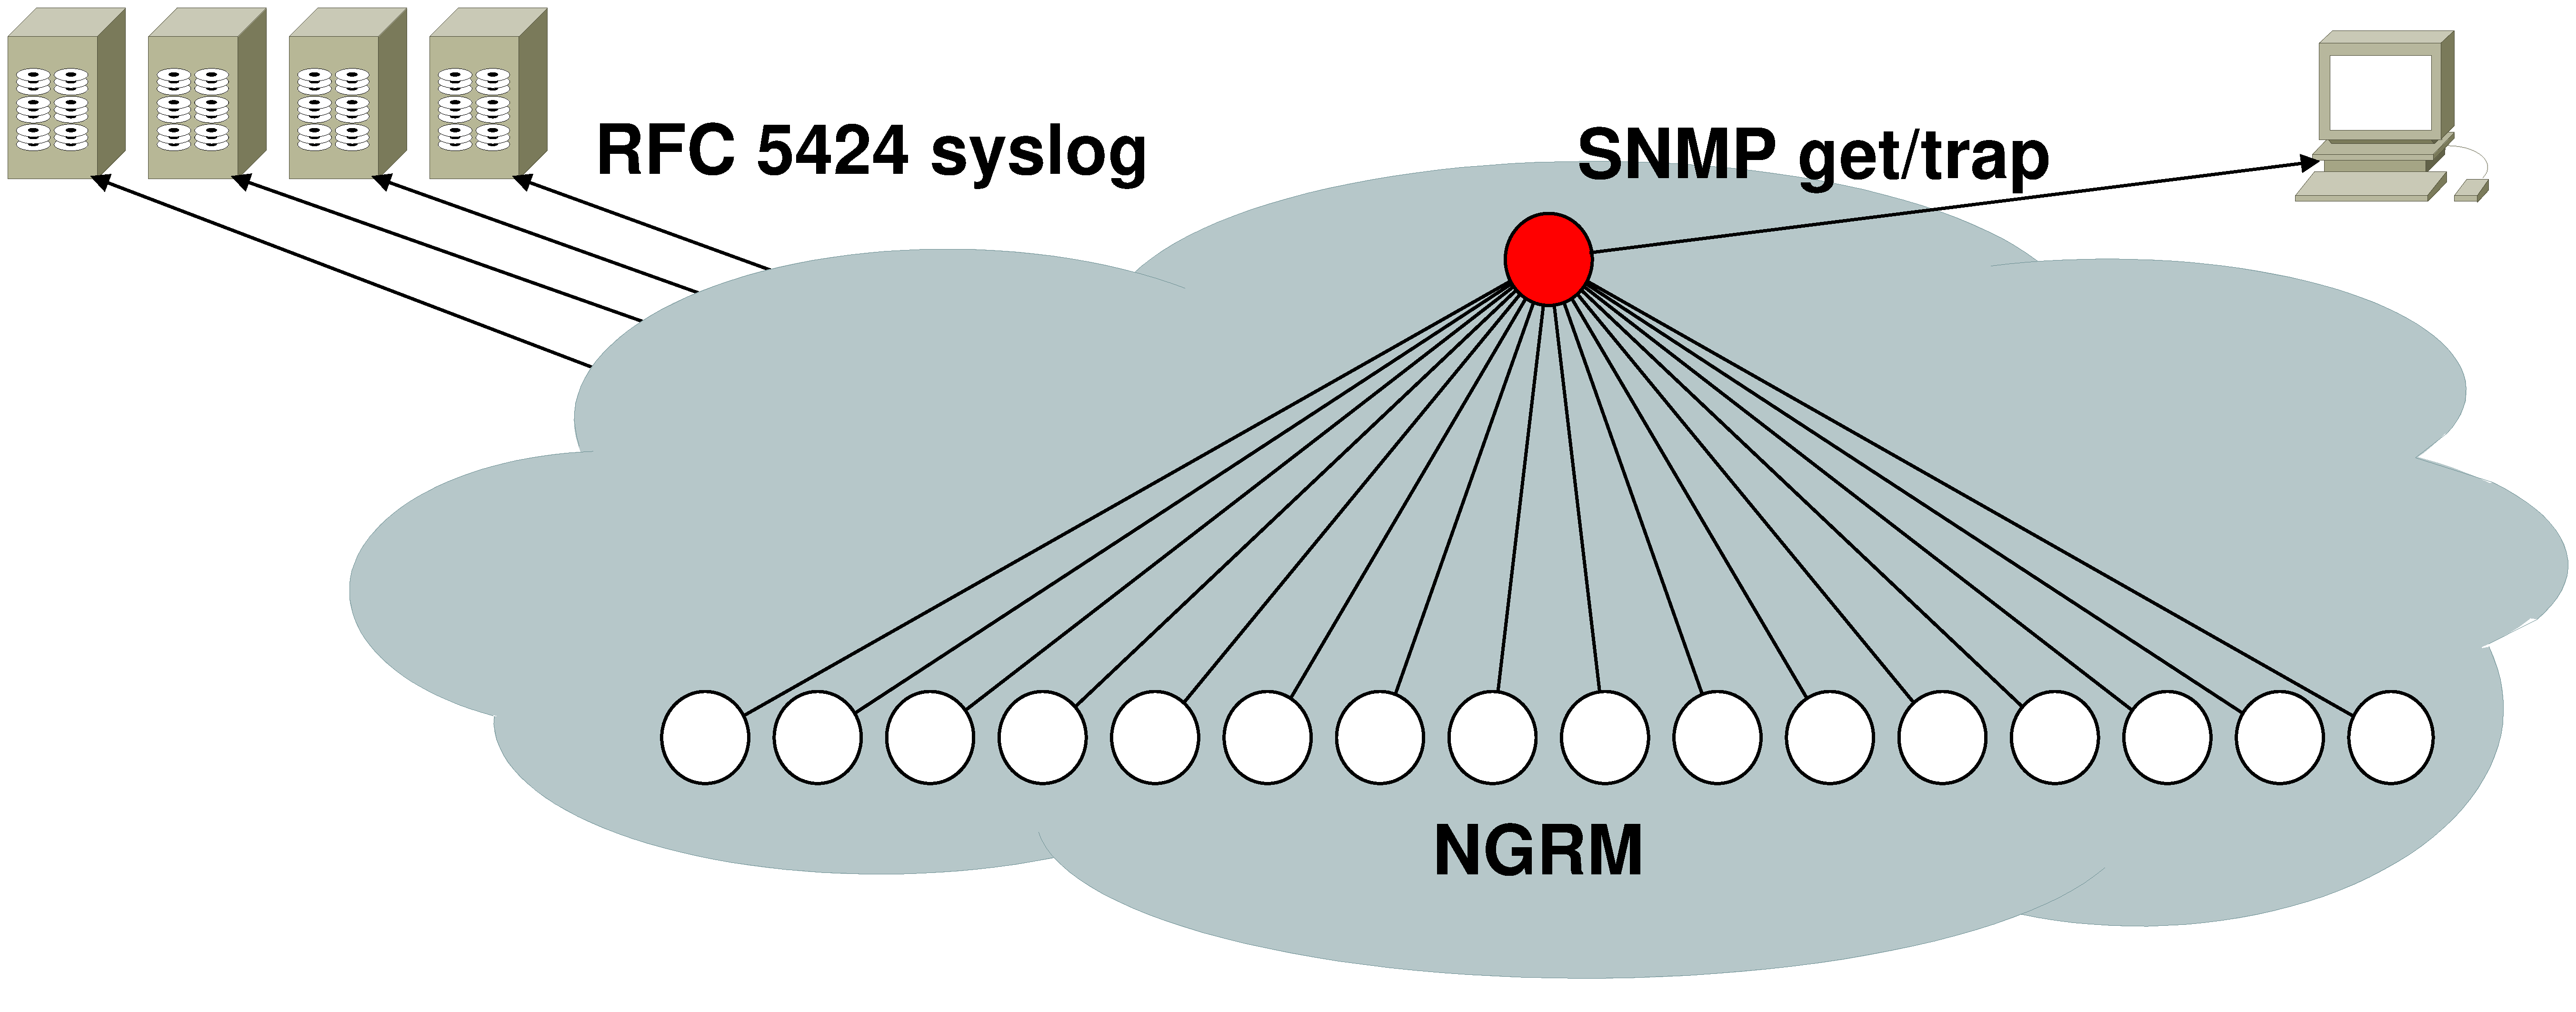
\includegraphics[scale=0.1]{../fig/mon_iface.eps}}
\caption{The \ngrm\ monitoring system interfaces with an external
enterprise monitoring system using SNMP, and with a persistent log
database using RFC 5424 structured syslog.}
\label{FigMonExt}
\end{figure}

\ngrm's integrated monitoring watches the health of its resources
to ensure that work is only launched on resources that are in good working
order and that appropriate action can be taken by the application, runtime,
or resource manager when things go wrong.
In order to mitigate the noise impact of monitoring on latency sensitive
bulk-synchronous workloads
(\ref{ReqsHiLevFun} req. 3.0), 
monitoring execution is synchronized by the comms layer's scheduling
trigger event.  Monitoring scalability is achieved through the comms
layer's event messaging and aggregation/reduction services.

Monitoring can be extended to cover emerging requirements
through the use of plugins
(\ref{ReqsHiLevFun} req. 3.1), and indeed seeks to be comprehensive
enough that it will supplant other noisey and less scalable monitoring
frameworks.
System administrators configure a monitoring plugin stack for the
root \ngrm\ instance which is inherited by sub-instances.
The owner of an instance, subject to some limitations, has the ability
to add or remove plugins from the plugin stack and tune the scheduling
event trigger period, according to application needs
(\ref{ReqsHiLevFun} req. 3.2).
Fault events generated by monitoring plugins within the job as well as
external, subscribed-to faults become part of the job record and
contribute to provenance of the result
(\ref{ReqsHiLevFun} req. 3.3).

Monitoring state is maintained on the session control node, and is
made accessible to other \ngrm\ subsystems.  Some fault events from
within the job are published by the control node to the parent, which
enables the parent to keep its state updated for resources "on loan"
to children.
% FIXME: do we need to copy state from parent to child on job exit
%also?
 
Monitoring is designed to interface with an external enterprise
monitoring system which might be used in an operations center setting
where data from \ngrm\ and other systems is aggregated and displayed.

Monitoring also interfaces with an external log database such
as Splunk\cite{Splunk} or Couchbase\cite{Splunk} where \ngrm\ monitoring
data can be correlated with other data collected there, facilitating
a more comprehensive post-mortem analysis than provided by the job record
alone.

\ngrm\ monitoring consists of three main components:
1) a plugin system which allows user and system defined code to execute
periodically to check for faults or take data samples, then generate
events,
2) a monitoring console which aggregates real-time monitoring data
within a session and makes it available to other \ngrm\ subsystems,

3) external interfaces to a site-provided persistent log database
and monitoring system.

\subsection{Monitoring Plugin System}

\begin{figure}
\begin{minipage}[b]{0.4\linewidth}
\fbox{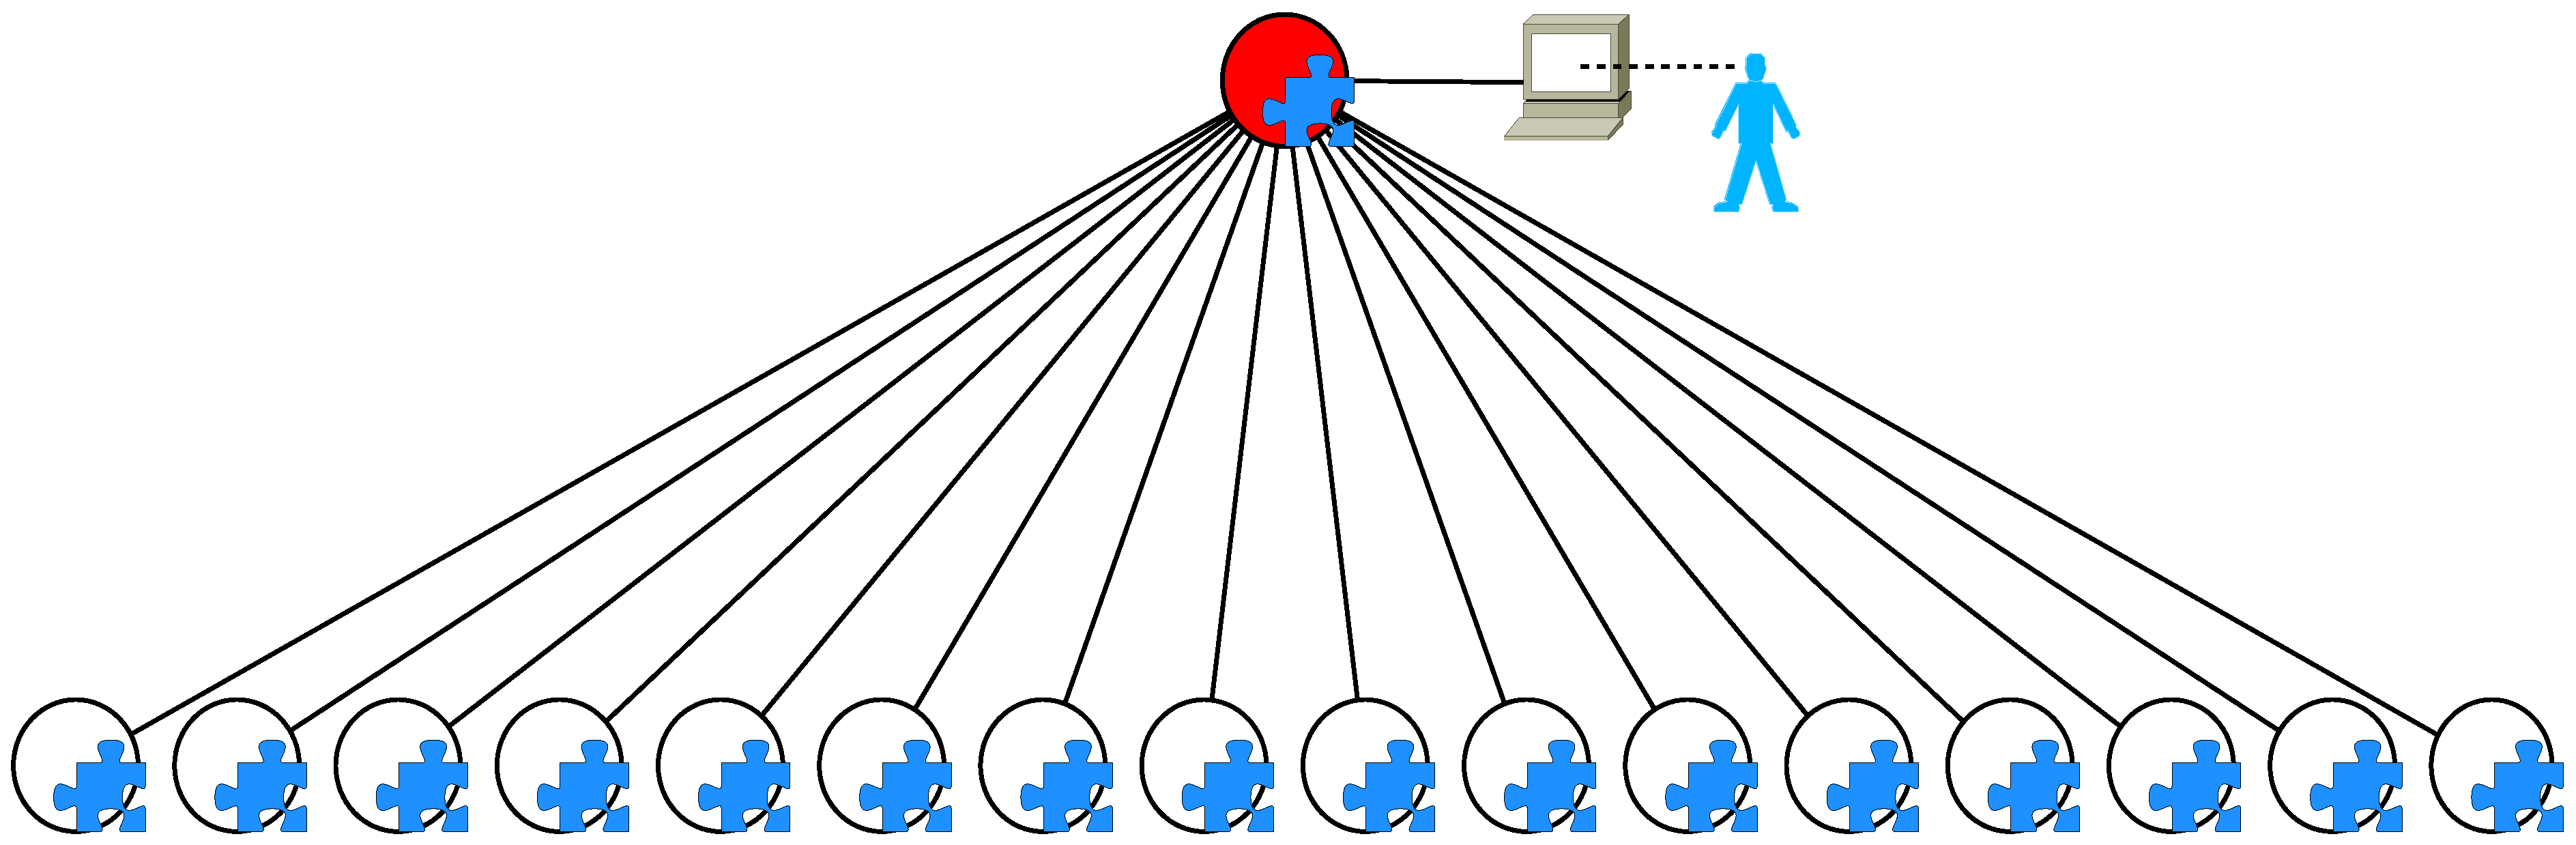
\includegraphics[scale=0.1]{../fig/mon_ex1a.eps}}
\end{minipage}
\hspace{1cm}
\begin{minipage}[b]{0.4\linewidth}
\fbox{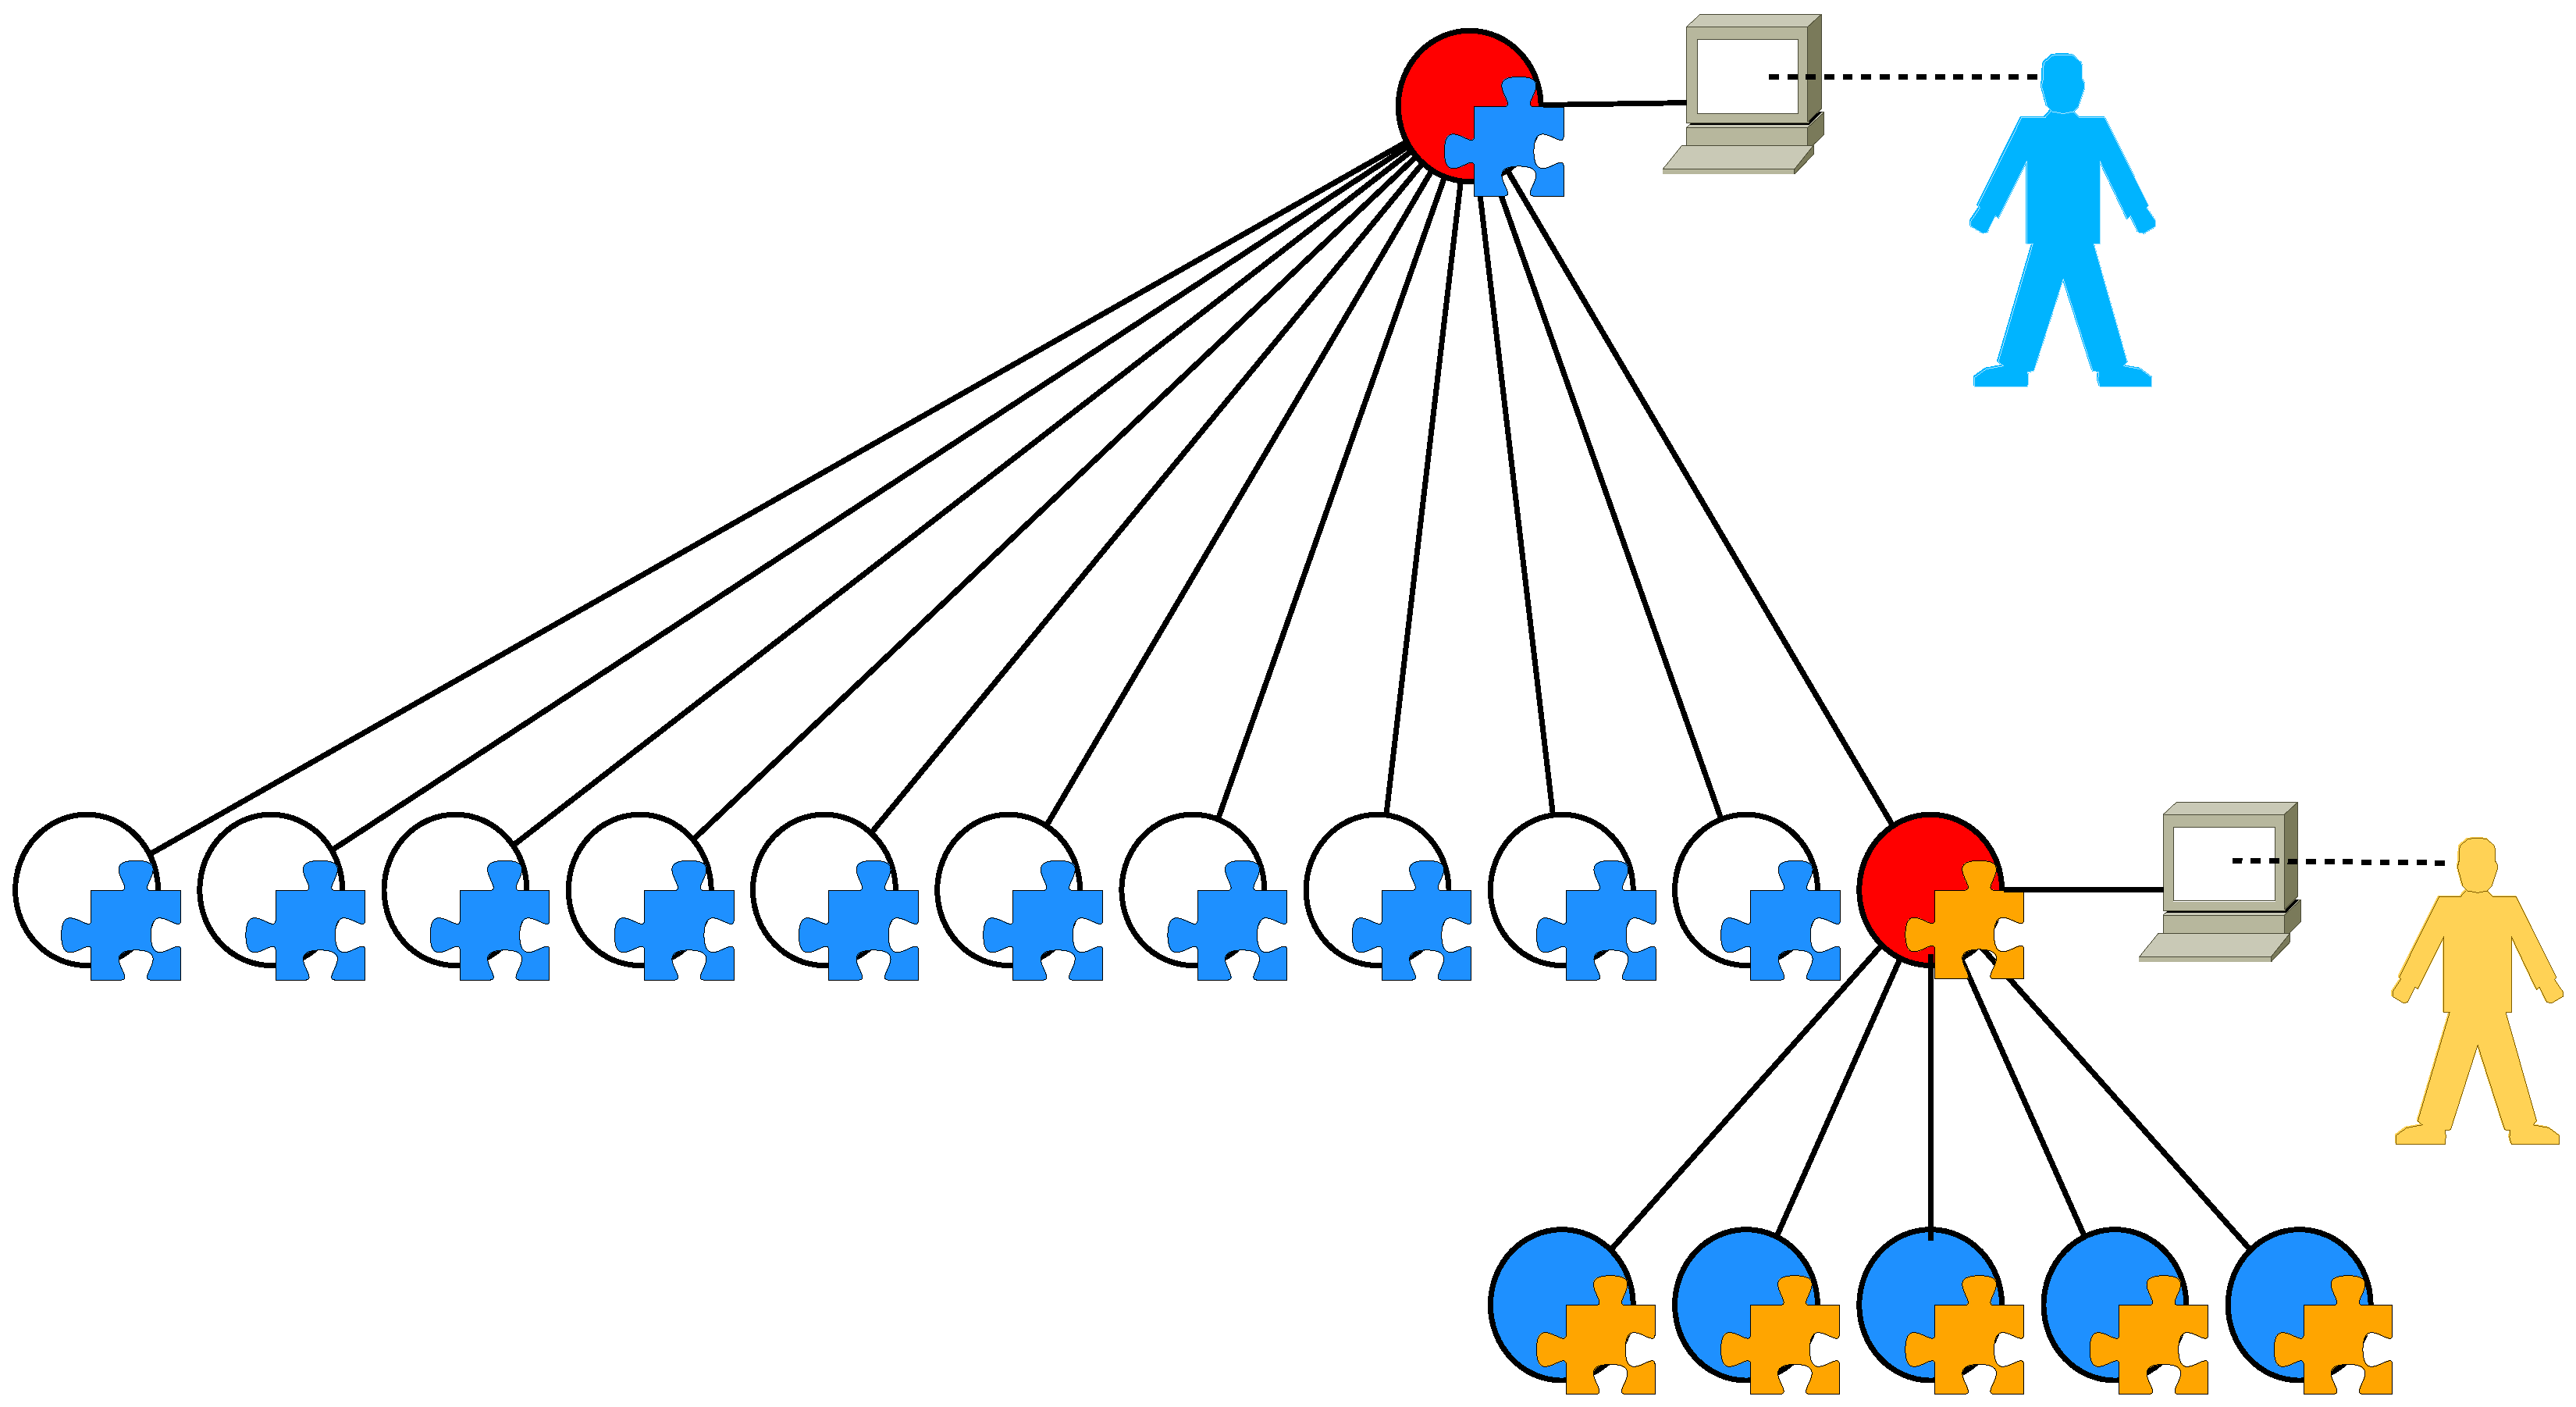
\includegraphics[scale=0.1]{../fig/mon_ex1b.eps}}
\end{minipage}
\caption{Monitoring follows the session/job hierarchy.
Control nodes (red) export a web-based monitoring console for each job.
The monitoring plugin stack (jigsaw pieces) is customizable for each job.
Plugin execution is coordinated by the job's scheduling trigger event.}
\label{FigMonEx1}
\end{figure}


The monitoring plugin system provides a facility for arbitrary code to be
periodically executed across a session.  To minimize disruption to
bulk-synchronous workloads, this execution is synchronized by the 
session scheduling trigger event.  The set of active plugins is
under the control of the session owner, with some reasonable
defaults provided that can be overridden.

%The details of the plugin structure is a design activity, however,
%an example of a possible solution is for plugins to take the form of
%Lua scripts loaded into the CMB state database
%(thus shared across the session) and executed in the context of
%a monitoring daemon with an embedded Lua interpreter.

Plugins have three main functions: data source, data reduction,
and data sink.  The data source function is driven by the scheduling
trigger and may directly publish events, for example if a monitored
value exceeds a threshold, or produce structured data for the
aggregation/reduction network.
The data reduction function aggregates structured data from instances
of the plugin's source function.
For example, a plugin that monitors the total amount of memory used
by the session might register a reduction function that takes the sum of
arriving samples.
Finally, plugins can register a function to sink data at the monitoring
console, rendering it for display, or at points in the session that interface
with the monitoring database for persistent storage.

\subsection{Monitoring Console}

The monitoring console runs on the session control node and provides
a centralized point for monitoring each session.
An HTTP interface is provided which includes links to the control nodes
of child sessions, thus the entire hierarchy of sessions can be navigated
from the root session with a web browser.
The console displays information about the session that comes directly
from the comms CMB, including its time of inception, node membership,
node liveness, users, and scheduling trigger period.

The set of active plugins and the views created by them are represented.
Events generated by plugins are displayed in a scrollable region.

All the information that is available via the monitoring console web page
is also available via command line tools to a shell user on the session
control node.

\subsection{Monitoring Database Interface}

The monitoring database will be a large, centralized, persistent database
that stores structured log data for analysis and data provenance.
Log data is generated by monitoring plugins, but may come from other sources
such as syslog, the \ngrm\ runtime, resource manager, or scheduler.

One reason this database is centralized is to allow queries
to be constructed that correlate failures or performance anomalies
across domains; for example, jobs running slow or producing incorrect
results because of file system problems.  The database will directly
benefit system administrators and suport staff who currently perform
these tasks manually.

By preserving contextual information surrounding the execution of a job,
we enable questions to be asked later on when the same job produces
different results.  This is a central goal of provenance.

The database will need some schema design in order to enable queries
that are operationally useful.  For example, RAS metrics may be obtained
on hardware component failures if we are careful to log enough information
to identify the component (e.g. a double bit memory error at address \#xxxx
versus a failure of dimm with model and serial number).

This effort will leverage the work of an in-progress LDRD
feasbility study\cite{LogLDRD}.

\subsection{Monitoring WBS}

\begin{longtable}{|p{1cm}|p{10.2cm}|p{1cm}|p{1cm}|p{1.8cm}|}\hline
  \textbf{Item} & \textbf{Description}
                & \textbf{Deliv}\footnote{SD = software drop,
                        DR = design review, V = viewgraphs, D = document}
                & \textbf{Weeks} & \textbf{Depend} \\
  \hline
  \hline
  \multicolumn{5}{|l|}{3.3. \textbf{Monitoring Plugin System}} \\
  \hline
  3.3.1.& Design/prototype plugin system including structured log format
	  and event naming.  (See also possible CIFTS/FTB tie-in in runtime).
          (See also Meyer monitoring project).
	& DR
	&
	& comms \\
  \hline
  3.3.2.& Implement plugin system.
        & SD
        &
        & 3.3.1 \\
  \hline
  3.3.3.& Document process for creating monitoring plugins.
        & D
        &
        & 3.3.1 \\
  \hline
  3.3.4.& Design/prototype a set of default plugins including plugins
          for instrumenting jobs to gather "implicit provenance" such as
          file accesses.
        & DR
        & 
        & 3.3.1 \\
  \hline
  3.3.5 & Implement set of default plugins.
        & SD
        &
        & 3.3.4 \\

  \hline
  \multicolumn{5}{|l|}{3.4. \textbf{Monitoring Console}} \\
  \hline

  3.4.1.& Design/prototype HTTP/REST monitoring console.
          (Long/Martinez Lorenz team)
          (See also Meyer monitoring project).
	& DR
	&
	& 3.3.1 \\
  \hline
  3.4.2.& Implement monitoring console.
	& SD
	&
	& 3.3.1, 3.4.1 \\
  \hline
  3.4.3.& Design/prototype Lorenz integration.
	  Think about how monitoring console integrates with the myllnl
	  dashboard experience.
          (Long/Martinez Lorenz team)
	& DR
	&
	& 3.4.1 \\
  \hline
  3.4.4.& Design/prototype skummee integration.
          How will \ngrm\ integrate with ops monitoring view?
          How will out of band monitoring (IPMI, DDN's, etc) integrate with
	  monitoring console?
          (Meyer monitoring project).
	& DR
	&
	& 3.4.1 \\
  \hline
  3.4.5.& Implement Lorenz/skummee integration.
	& SD
	&
	& 3.4.3, 3.4.4 \\
  \hline
  \multicolumn{5}{|l|}{3.5. \textbf{Monitoring Database Interface}} \\
  \hline
  3.5.1.& Study available NoSQL databases for 100K node scalability
          and appropriate query interface.
          Use offline log data to investigate system diagnostic capability
          and prototype queries.
          (Gamblin/Mohror HPC Data Analytics FY12 LDRD)
        & V
        & 
        & LDRD \\
  \hline
  3.5.2.& Implement prototype database tied to live log sources.
          Study scalability and develop queries.
          (Gamblin/Mohror HPC Data Analytics FY12 LDRD)
          (See also: Faaland SPLUNK deployment).
        & DR
        & 
        & 3.5.1 \\
  \hline
  3.5.3.& Design/prototype access-role based security.
        & DR
        & 
        & 3.5.2 \\
  \hline
  3.5.4.& Design/prototype schemas and queries for reporting
          RAS metrics of interest to center management.
        & DR
        & 
        & 3.5.2 \\
  \hline
  3.5.5.& Design/prototype procedure for sanitizing and releasing data
	  for research study and citation.
        & DR
        & 
        & 3.5.2 \\
  \hline
  3.5.6.& Design/prototype schema for job logs and queries for
          associating job data, system log data, etc..
        & DR
        & 
        & RM, 3.5.2 \\
  \hline
  3.5.7.& Implement database.
        & SD
        & 
        & 3.5.2, 3.5.3, 3.5.4, 3.5.5, 3.5.6 \\
  \hline
\end{longtable}


